% block_diagram_annotated.tex -- inference-pipeline diagram with an enlarged
% legend. Overlays ../figures/block_diagram.png (2100 x 576 px): covers the
% original small legend (x 910-1355, y 520-566 px from the top) and draws a
% larger one beside the light-blue "computed once" boxes (y 311-498 px),
% using the diagram's own colours.
% Build: pdflatex block_diagram_annotated.tex
\documentclass[tikz,border=0pt]{standalone}
\usepackage[T1]{fontenc}
\usepackage[default]{sourcesanspro}
\definecolor{boxedge}{RGB}{42,120,214}
\definecolor{boxfill}{RGB}{219,232,249}
\definecolor{legtext}{RGB}{82,81,78}
\newlength\pxu
\setlength\pxu{0.01833cm}   % 2100 px -> 38.5 cm, about its printed width
\begin{document}
\begin{tikzpicture}[x=\pxu, y=\pxu]
  \node[anchor=south west, inner sep=0pt] at (0,0)
    {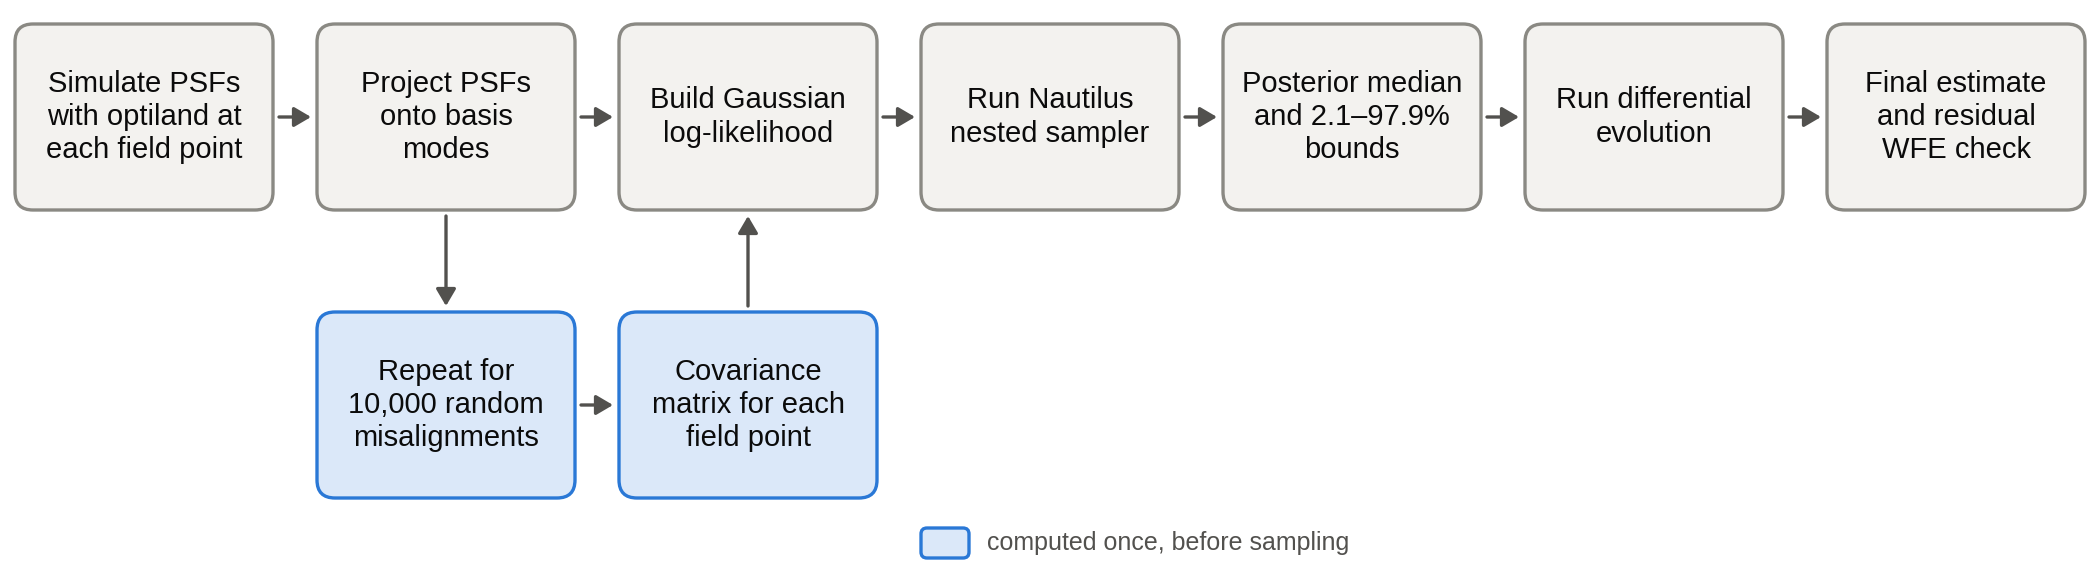
\includegraphics[width=2100\pxu]{../figures/block_diagram.png}};
  % Cover the original legend (image y measured from the top; H = 576)
  \fill[white] (910,{576-566}) rectangle (1355,{576-520});
  % Enlarged legend, vertically centred on the light-blue boxes
  \draw[boxedge, fill=boxfill, line width=2.5pt, rounded corners=6pt]
    (950,{576-430}) rectangle (1040,{576-380});
  \node[anchor=west, text=legtext, font=\fontsize{20}{24}\selectfont]
    at (1065,{576-405}) {computed once, before sampling};
\end{tikzpicture}
\end{document}
